\clearpage
\section{Background Estimation}
\label{sec:bkgEst}

\subsection{Exclusive WW}
\par As shown at the end of Section~\ref{sec:theory} there are three diagrams that contribute 
to the exclusive WW process. Although Herwig++ models the purely elactic events well, there are 
no MC that model SD and DD processes. To estimate the SD and DD contributions we study di-muon
events in data that pass the exclusivity cut and that have $\mll>160$ GeV to reduce di-muons 
from WW decays and Drell-Yan. The remaining Drell-Yan contribution in this region is estimated 
with MC and subtracted. All other backgrounds are considered as well but the major contributions are observed 
to be from inclusive WW, exclusive WW and Drell-Yan. Inclusive WW and Drell-Yan estimations 
are scaled with appropriate MFs to account for the MC mismodelling of the underlying event.
There is no need to apply MF to exclusive WW and exclusive di-muon estimates because there 
is no underlying event in these processes. 

\par After all the backgrounds are subtracted the remaining events are a good estimation of 
the sum of purely elastic, single dissociative and double dissociative di-muons. We introduce 
the

\begin{equation}
\mbox{Flux Factor} = \frac{N_{data} - N_{DY,etc}}{N_{elastic}}
\end{equation}

which quantifies the SD and DD contributions. Detailed studies concerning this factor can 
be found in Ref~\cite{CMSmumu}. A flux factor of 1.0 indicates that there is negligible SD 
and DD contributions to the exclusive di-muons. Table~\ref{table:flux} shows the results 
of studying di-muon events in data. A flux factor of $2.99\pm0.21$ is obtained, in which the 
uncertainty is only statistical. This shows that the SD and DD contributions are non-negligible.  

\begin{table}
\centering
        \resizebox{.4\textwidth}{!}{
\providecommand{\cutflowTitle}{hsg3}
\begin{tabular}{l|r}
\hline
 & Count \\
\hline\hline
Observed & 234 \\
Predicted Elastic $ll$ & 72.0 \\
MF-Scaled Drell-Yan & 16.2 \\
MF-Scaled Inclusive WW & 0.4 \\
MF-Scaled Exclusive WW & 0.82 \\
\hline
Flux Factor & $2.99\pm0.21$ \\
\end{tabular}
}
\caption{Results for the flux factor study on exclusive di-muons. A large flux factor 
implies that the contribution of SD and DD processes is non-negligible.}
\label{table:flux}
\end{table}

The diagrams that contribute to exclusive di-leptons are identical to the diagrams that contribute to 
exclusive WW. Thus, we can use the flux factor obtained from the di-muon study to estimate the 
SD and DD contributions in exclusive WW. We scale the Herwig++ estimation with 2.99 
to get the expected final exclusive WW yield, which turns out to be $1.25\pm0.02$. 

\subsection{Inclusive WW}
\par Inclusive WW are estimated using MC listed in Table~\ref{table:background}. A control region is 
used to assess the performance of these MC. The control region is defined as follows: Events that pass all 
the signal region cuts up to the $\ptll>30$ GeV cut are required to have $55<\mll<110$ GeV and 
$\dfll<2.6$ and have no jets. The 0-jet requirement suppresses \ttbar\ contribution. These selection criteria 
for this region are similar to the 0-jet WW control region detailed in Ref.~\cite{ATLASCONF2014060}. 
We notice that it is necessary to scale WW MC estimate by a factor of 1.22 to achieve data/MC agreement. 
This factor was also introduced in the \hwwll\ studies in Ref.~\cite{ATLASCONF2014060}. 
The exclusivity cut is then imposed after all these requirements are fulfilled and the scale 
factor has been applied.
Figure~\ref{fig:wwCR} shows key kinematic distributions in this control region after scaling MC with 1.22.
Table~\ref{table:wwCR} shows the corresponding MC estimated yields and observed event yields.
Figure~\ref{fig:exclwwCR} shows the $\Delta z_1$ distribution after applying the 1.22 scale factor on 
the inclusive WW, an MF on the inclusive WW and a flux factor on the exclusive WW processes.

\begin{figure}[!h]
\centering
\begin{tabular}{c}
	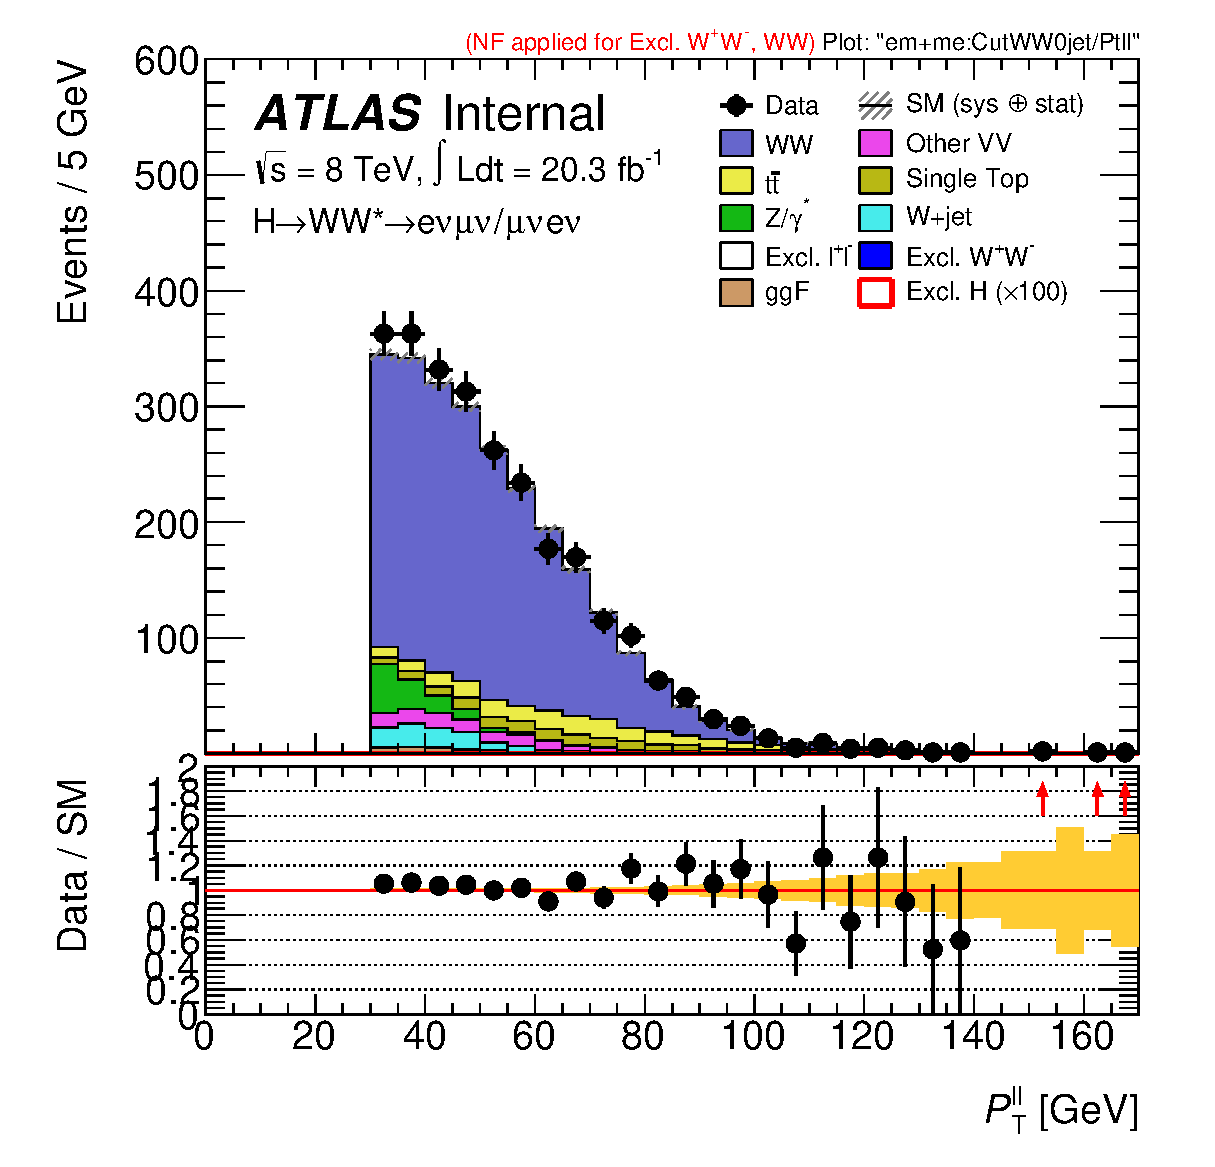
\includegraphics[width=0.5\linewidth]{emme_CutWW0jet_Ptll_mh125_lin.eps}
	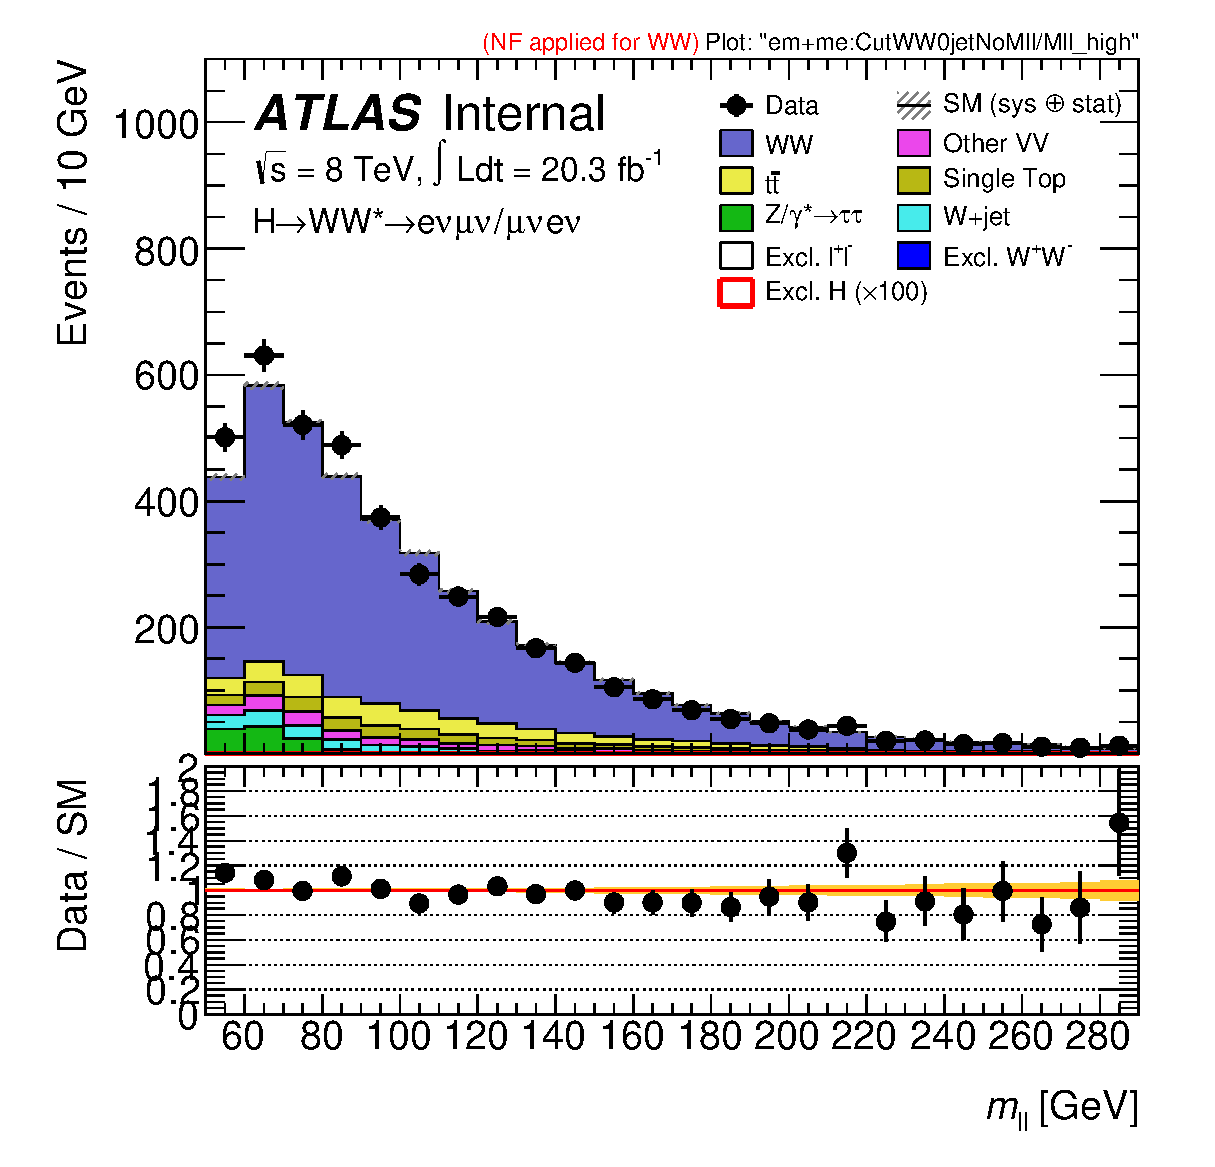
\includegraphics[width=0.5\linewidth]{emme_CutWW0jetNoMll_Mll_high_mh125_lin.eps}\\
	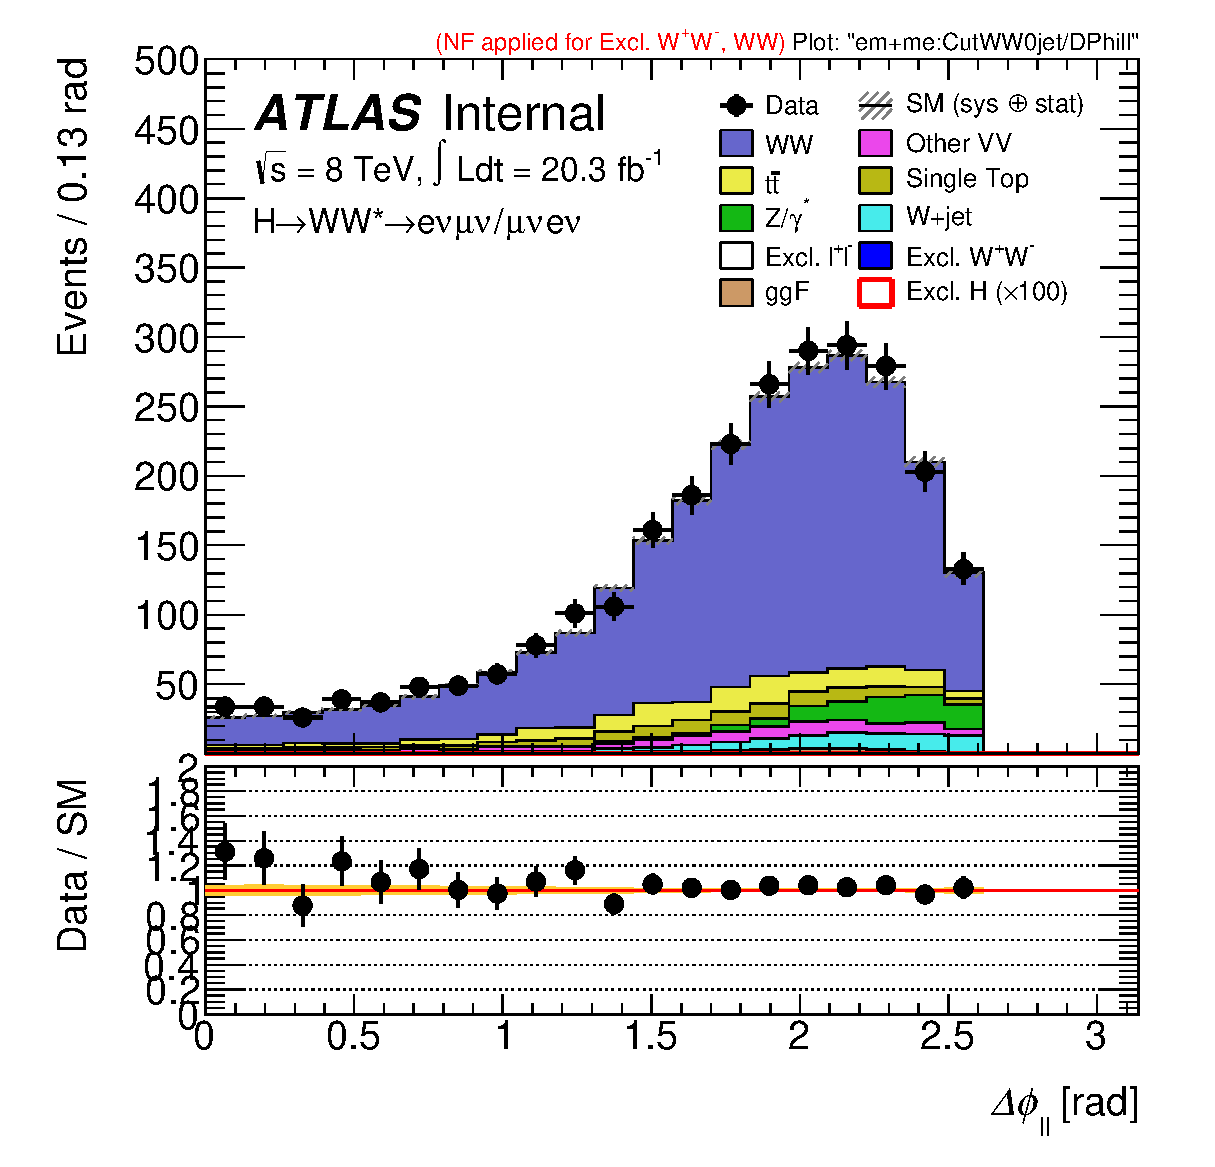
\includegraphics[width=0.5\linewidth]{emme_CutWW0jet_DPhill_mh125_lin.eps}
	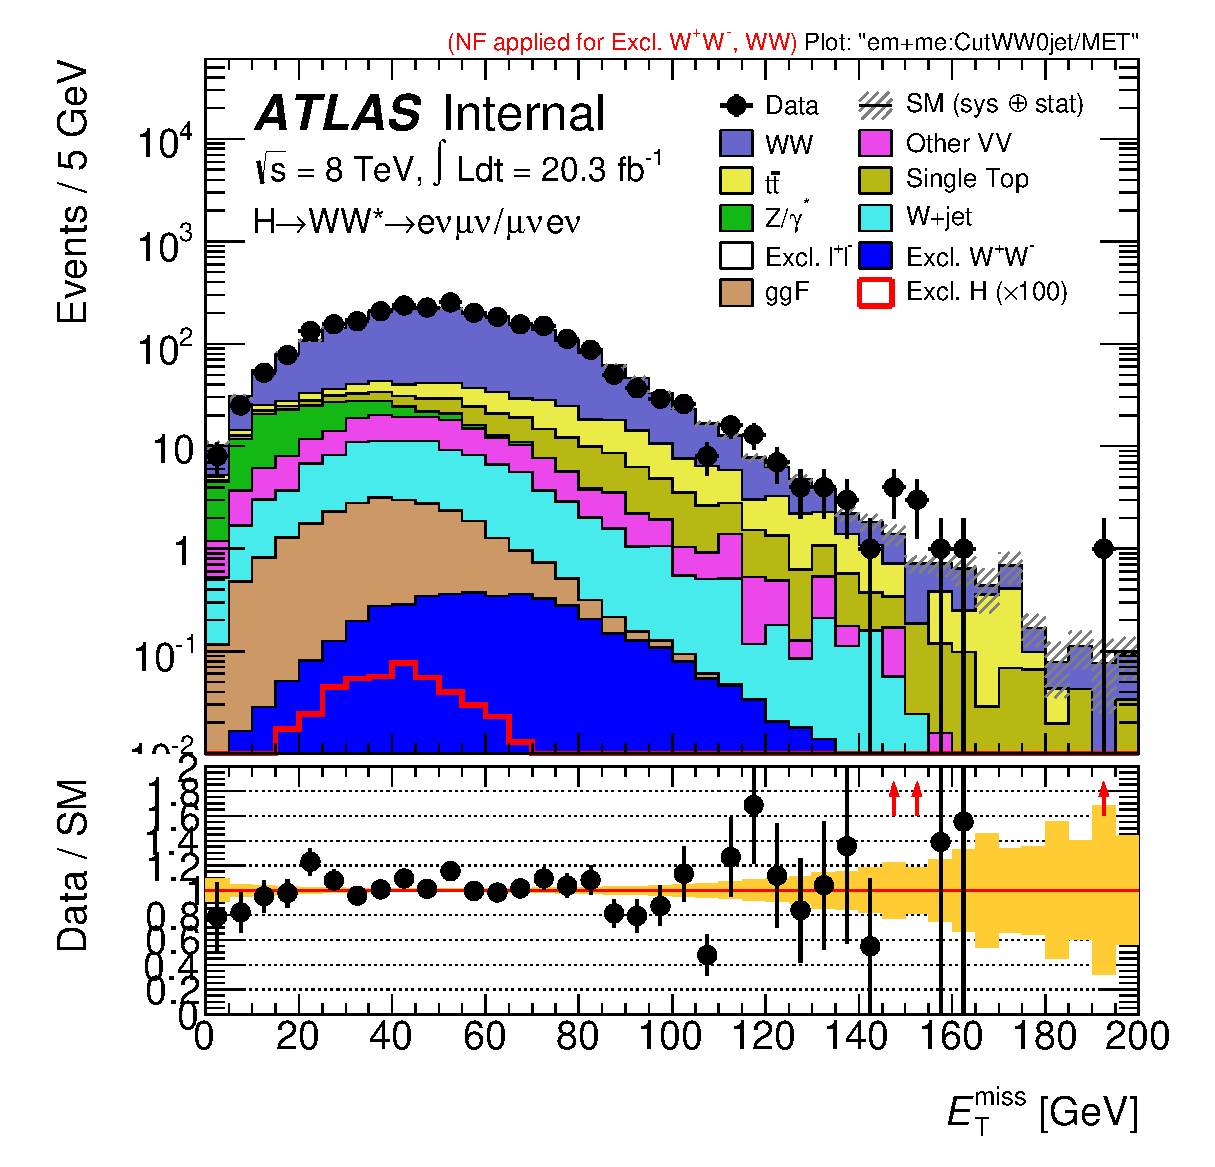
\includegraphics[width=0.5\linewidth]{emme_CutWW0jet_MET_mh125_log.eps}\\
	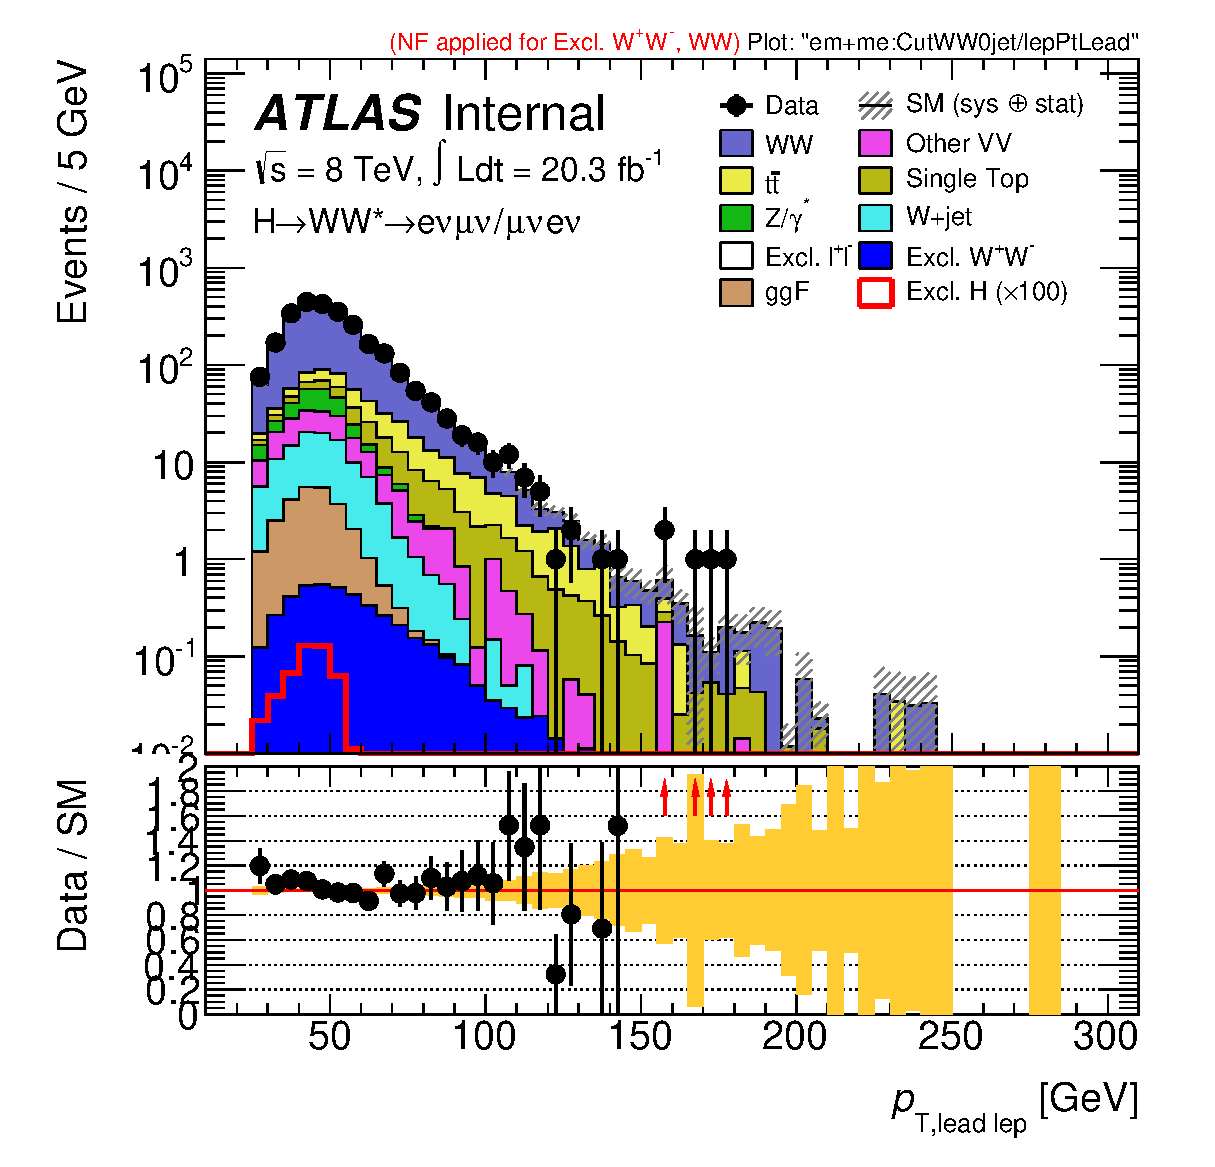
\includegraphics[width=0.5\linewidth]{emme_CutWW0jet_lepPtLead_mh125_log.eps}
	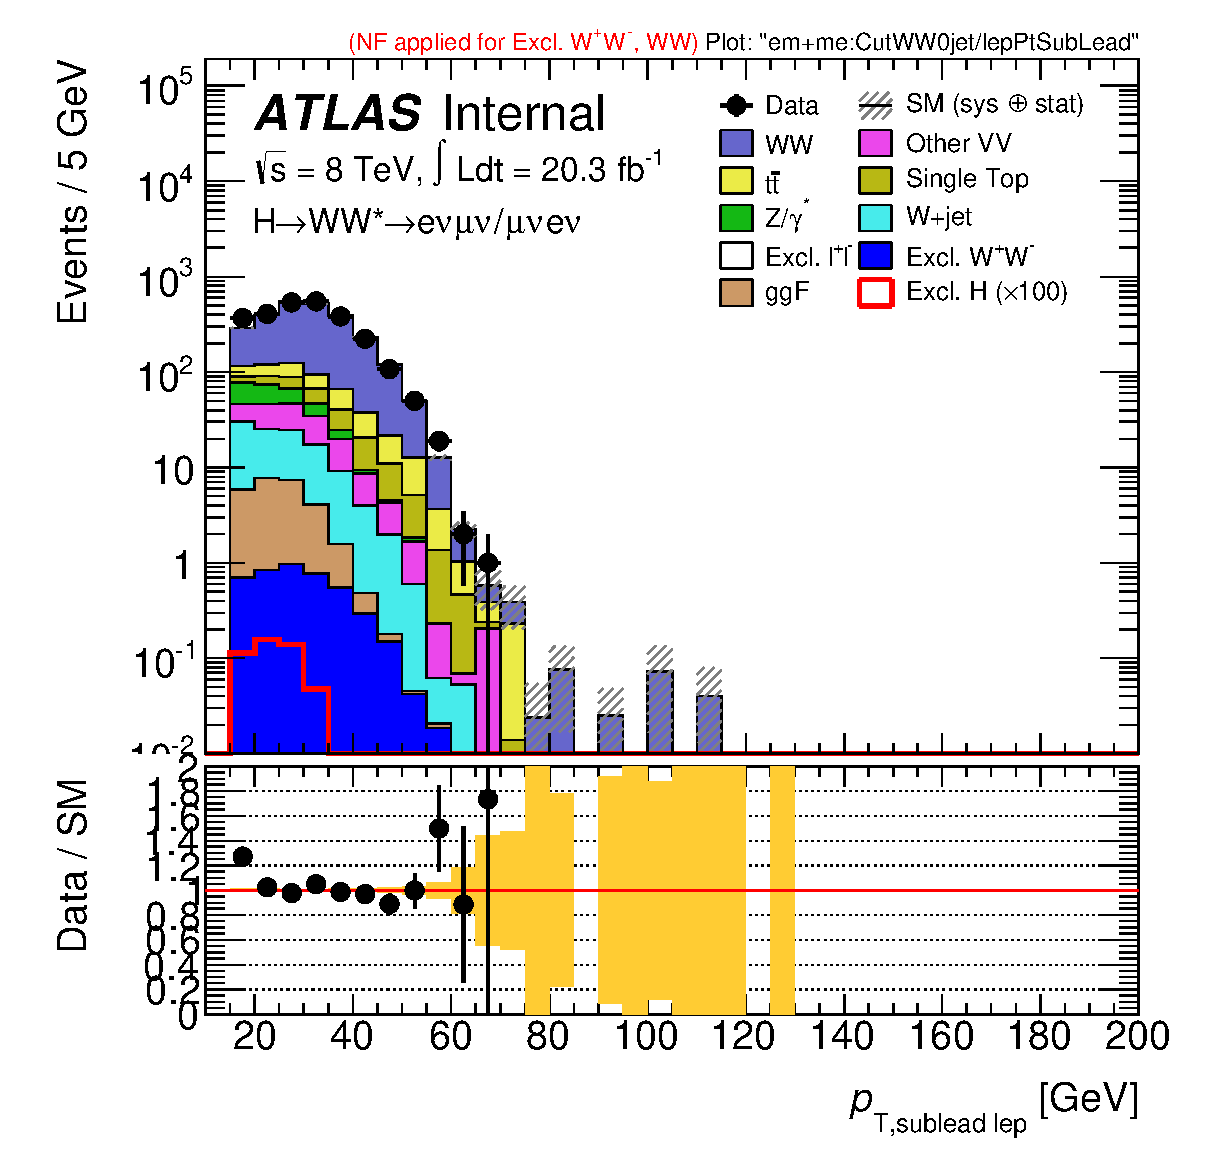
\includegraphics[width=0.5\linewidth]{emme_CutWW0jet_lepPtSubLead_mh125_log.eps}\\
\end{tabular}
\caption{Key kinematic distributions in the WW control region before the exclusivity cut is imposed.}
\label{fig:wwCR}
\end{figure}

\begin{figure}[!h]
\centering
	\includegraphics[width=0.5\linewidth]{emme_CutWW0jet_trkdz0_asymm_mh125_log.eps}
\caption{Exclusivity variable $\Delta z_1$ after an MF has been applied on the inclusive WW process, 
and a flux factor has been applied on the exclusive WW process.}
\label{fig:exclwwCR}
\end{figure}

\begin{table}
\centering
        \resizebox{\textwidth}{!}{
\providecommand{\cutflowTitle}{}
\begin{tabular}{l||rrr|rrr}
Cuts & $WW$ & Excl. $W^{+}W^{-}$ & Other Bkgs & Total Bkg. & Observed & Data/MC \\
\hline\hline
WW CR [$55<m_{\ell\ell}<110$ GeV,$\Delta\phi_{\ell\ell}<2.6$] & 2755.90 $\pm$ 9.99 & 1.48 $\pm$ 0.02 & 9750.32 $\pm$ 153.94 & 12513.27 $\pm$ 154.26 & 12176 & 0.97 $\pm$ 0.01 \\
0 jet & 1946.03 $\pm$ 8.42 & 4.35 $\pm$ 0.05 & 795.62 $\pm$ 133.21 & 2750.17 $\pm$ 133.47 & 2644 & 0.96 $\pm$ 0.05 \\
1 mm Exclusive & 1.21 $\pm$ 0.14 & 2.39 $\pm$ 0.03 & 0.47 $\pm$ 0.32 & 4.07 $\pm$ 0.35 & 9 & 2.21 $\pm$ 0.76 \\
\end{tabular}
}
\caption{Estimated and observed events in the WW CR.}
\label{table:wwCR}
\end{table}

\par The inclusive WW contribution to the signal region turns out to be $0.77\pm0.10$ events.

\subsection{Other Backgrounds}
\par The rest of the backgrounds are estimated using MC, except for the W+jets. Events are selected in data 
that have exactly two leptons, one tightly identified and the other loosely but not tightly identified. These 
events turn out to be 85\% W+jets. All other backgrounds are subtracted from this data sample to obtain a better 
estimation of the W+jets in data. All the backgrounds that use MC are applied appropriate MFs except for exclusive 
dileptons. A flux factor of 2.99 is applied to the exclusive dileptons estimate, which only estimates purely 
elastice processes. A list of all the MC generators used are listed in Table~\ref{table:background}. 
We estimate $0.10\pm0.06$ from all these backgrounds.
